\chapter{Diseño e implementación} % Main chapter title

\label{Chapter3}

En este capítulo se describe el diseño e implementación de los diferentes módulos de software y hardware del sistema, como así también las diferentes herramientas utilizadas.

El sistema propuesto reemplazará al sistema actual de SURIX, el mismo que es un llamador cableado que se conecta en uno de los puertos de accesorio que tiene el terminal de sala, y donde tanto el micrófono como el parlante se encuentra ubicado en dicho terminal.

El nuevo sistema cambia la ubicación del micrófono al dispositivo llamador, de manera que ahora está más cerca del paciente. De esta forma se mantiene el parlante en la terminal de sala, mejorando así la comunicación.

El micrófono seleccionado utiliza la interfaz de audio digital PDM, que es compatible con el procesador elegido dispone de un periférico para controlar micrófonos con este tipo de interfaz.

La comunicación entre el dispositivo Bluetooth y la terminal de llamada se realiza a  través de una interfaz UART, que está disponible en los puertos de accesorios de la terminal de llamada del sistema anterior.
En este sistema el audio se transmite codificado en PCMU, para mantener compatibilidad con el anterior sistema.


%----------------------------------------------------------------------------------------
%	SECTION 1
%----------------------------------------------------------------------------------------
\section{Hardware}

Aunque la idea inicial era diseñar dos placas electrónicas distintas: Una para el dispositivo llamador y, otra para el lado de la terminal sala, como una placa de extensión de la placa principal de dicha terminal, la terminal de llamada, luego de realizar los Diagramas esquemáticos se vio conveniente diseñar un solo diagrama que sirve para ambos dispositivos. 

Los principales componentes de esta placa son:

\begin{itemize}

\item Un modulo bluetooth LE MDBT42Q-512KV2, que internamente cuenta con un microcontrolador NRF52832 ARM Cortex-M4 de la empresa Nordic, mismo que cumple con las especificaciones de bluetooth LE 5.2, 5.2, 5 y 4.2. Se eligió este módulo porque ya cuenta con una antena de manera que ya no es necesario diseñar la misma. Este módulo se aprecia en la figura \ref{fig:MDBT42}, y sus principales características se resumen en la tabla \ref{tab:CaracteristicasMDBT42}.

\item Un micrófono digital con interfaz PDM SDM0401-RS261-G04, seleccionado por su bajo costo y tamaño. Este micrófono se puede observar en la figura \ref{fig:mic} y sus características se muestran en la tabla \ref{tab:caracteristicasMic}.

\item El circuito cuenta con la posibilidad de incluir hasta cuatro pulsadores para interacción con el usuario, en el dispositivo llamador, dicho número puede variar de acuerdo a las versiones de llamador que tiene actualmente la empresa, que varían de 2 a 4 pulsadores según el modelo. También contará con dos LEDs para que el usuario tenga retroalimentación del funcionamiento del dispositivo.

\end{itemize}

\begin{figure}[htpb]
	\centering
	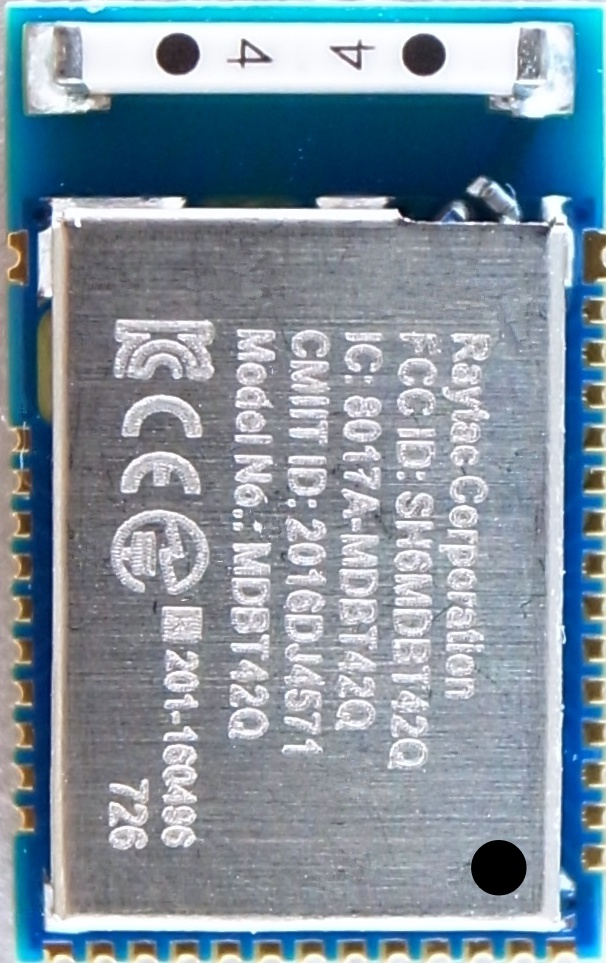
\includegraphics[scale=0.15]{./Figures/MDBT42Q.jpg}
	\caption{Modulo MDBT42Q-512KV2}
	\label{fig:MDBT42}
\end{figure}

\begin{table}[h]
	\centering
	\caption[Características modulo MDBT42Q-512KV2]{Tabla de características modulo MDBT42Q-512KV2}
	\begin{tabular}{l c}    
		\toprule
		\textbf{Característica} 	 & \textbf{Valor}\\
		\midrule
		Tamano (mm)                                                        & 8.8 x 13.8 x 1.8       \\
\begin{tabular}[c]{@{}l@{}}Especificacion\\ Bluetooth\end{tabular} & BT50.1 / BT5.0 / BT4.2 \\
Antena                                                             & Incluida en el modulo  \\
\begin{tabular}[c]{@{}l@{}}Longitud de\\ cobertura\end{tabular}    & \textgreater 80 m      \\
RAM                                                                & 64 Kbytes              \\
Flash                                                              & 512 Kbytes             \\
Pines GPIO                                                         & 32						\\
		\bottomrule
		\hline
	\end{tabular}
	\label{tab:CaracteristicasMDBT42}
\end{table}

\begin{figure}[htpb]
	\centering
	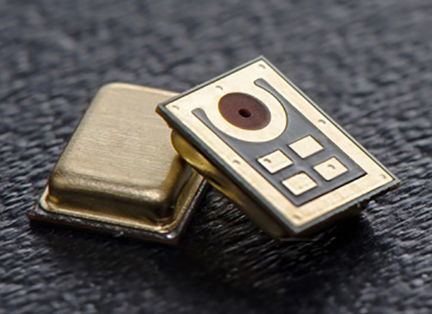
\includegraphics[scale=0.3]{./Figures/mic.png}
	\caption{Micrófono SDM0401-RS261-G04}
	\label{fig:mic}
\end{figure}

\begin{table}[h]
	\centering
	\caption[Características micrófono SDM0401-RS261-G04]{Tabla de características micrófono SDM0401-RS261-G04}
	\begin{tabular}{l c}    
		\toprule
		\textbf{Característica} 	 & \textbf{Valor}\\
		\midrule
		\begin{tabular}[c]{@{}l@{}}Voltaje de\\ alimentacion\end{tabular} & 1.8 V            \\
\begin{tabular}[c]{@{}l@{}}Frecuencia de\\ reloj\end{tabular}     & 2.4 MHz          \\
Directividad                                                      & Omni-Direccional \\
		\bottomrule
		\hline
	\end{tabular}
	\label{tab:caracteristicasMic}
\end{table}

Con estos componentes se diseño un diagrama esquemático, a partir del cual se diseñó la placa del dispositivo llamador, que se muestra en la figura \ref{fig:esquematico}.

\begin{figure}[htpb]
	\centering
	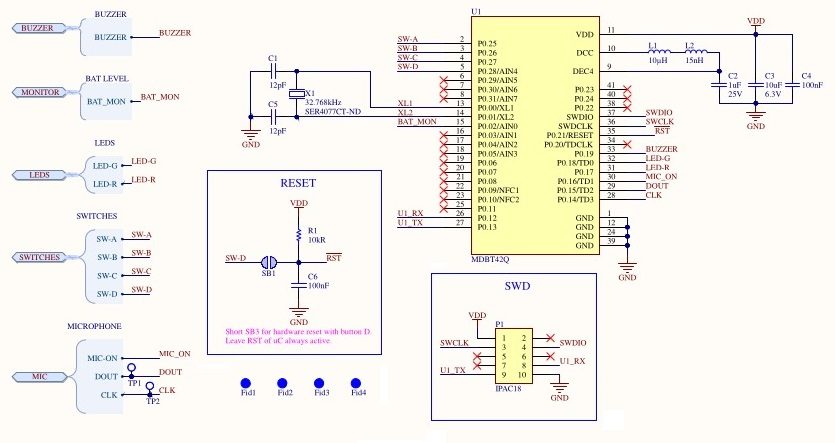
\includegraphics[scale=0.6]{./Figures/esquematico.jpeg}
	\caption{Diagrama esquemático para placas Bluetooth}
	\label{fig:esquematico}
\end{figure}

A partir de este de diagrama se diseñó la placa del dispositivo llamador, que se muestra a en la figura \ref{fig:pcb}.

\begin{figure}[htpb]
	\centering
	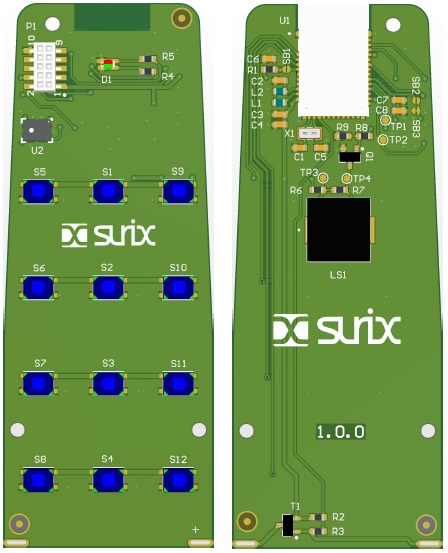
\includegraphics[scale=0.4]{./Figures/placas.jpeg}
	\caption{Placa dispositivo llamador}
	\label{fig:pcb}
\end{figure}

La fabricación de esta placa se ha encargado a una empresa China de confianza de SURIX, motivo por el cual este proceso se retrasó y no es posible mostrarla físicamente.

Para que el circuito pueda ser utilizado tanto en el llamador como del lado de la terminal de llamada se ha previsto que el circuito pueda ser alimentado, por la terminal de sala de SURIX en la terminal de llamada, o por 2 baterías tipo AAA en el dispositivo llamador, estas últimas se escogieron debido principalmente a la facilidad de adquirirlas en el mercado y su relativamente bajo costo.

La placa del dispositivo llamador se aloja dentro de un gabinete plástico, el cual se muestra en la figura \ref{fig:gabinete}, sin embargo este se modificara segun las necesidades de SURIX.

\begin{figure}[htpb]
	\centering
	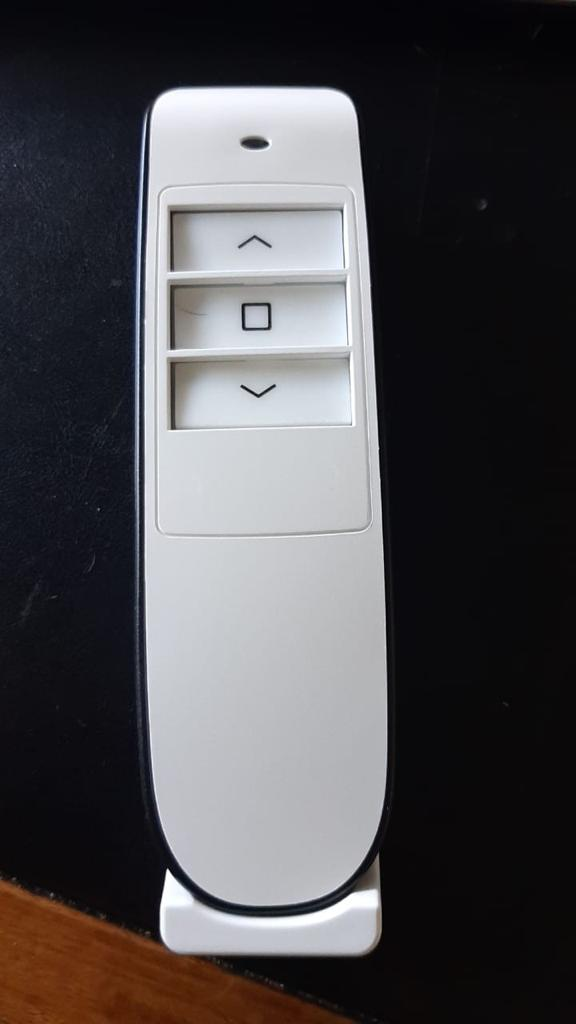
\includegraphics[scale=0.25]{./Figures/gabinete.jpeg}
	\caption{Prototipo gabinete del dispositivo llamador}
	\label{fig:gabinete}
\end{figure}

%----------------------------------------------------------------------------------------
%	SECTION 2
%----------------------------------------------------------------------------------------

\section{Software}

Para cumplir con los objetivos del trabajo, se dividió el software en tres componentes:

\begin{itemize}

\item El primero que trabaja en bare metal y controla el dispositivo llamador

\item El segundo también trabaja en bare metal y controla la placa de la terminal de llamada.

\item El tercero es un módulo que se agrega al software del sistema hospitalario de SURIX, el cual trabaja con el sistema operativo FreeRTOS.

\end{itemize}

La implementación de dichos componentes se describen en los apartados \ref{subsec:SoftLlam}, \ref{subsec:SoftCentral} y \ref{subsec:SoftControl}.

\subsection{Software del dispositivo llamador}
\label{subsec:SoftLlam}

En el desarrollo de este firmware se utilizó el paquete de desarrollo de software de Nordic para su familia de microcontroladores 52, de la que es parte el microcontrolador utilizado. Se utilizó la versión 17 de este paquete de desarrollo,  junto con el softdevice s132, que es la implementación más moderna del stack Bluetooth que nos ofrece esta versión del paquete de desarrollo de Nordic.

Este software se desarrolló utilizando el compilador GCC que proporciona ARM junto con las herramientas de línea de comandos nRF de Nordic.

Para el desarrollo de este firmware se realizó un diagrama de bloques que describe de manera general el comportamiento de este software. El diagrama mencionado se muestra en la figura \ref{fig:DiagramaSoftLlam}.

\begin{figure}[htpb]
	\centering
	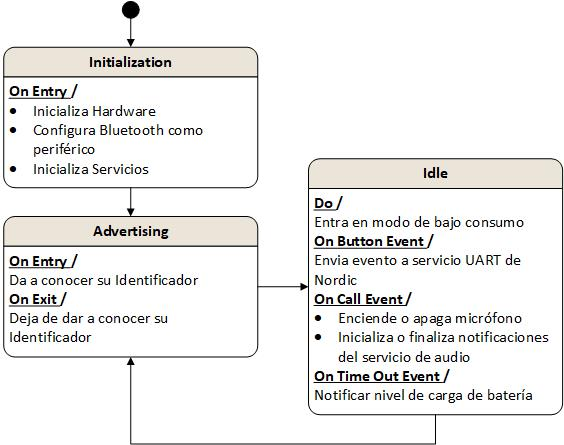
\includegraphics[scale=0.8]{./Figures/DCaller.jpeg}
	\caption{Diagrama de bloques del software del llamador}
	\label{fig:DiagramaSoftLlam}
\end{figure}

Este dispositivo al ser productor de datos en la comunicación Bluetooth, y debido a que sólo se conecta a la central receptora del terminal de sala, se lo programa para que en la conexión cumpla el rol de periférico, definido en el estándar de Bluetooth LE. 

Al estar programado de esta manera el dispositivo inicialmente se programó para que, entre los datos que lo identifican, envíe el identificador único del microcontrolador, durante el proceso de advertising, en el cual se da a conocer a todos los dispositivos bluetooth que están escaneando el ambiente cercano. Dicho identificador usará la central receptora del Bluetooth para decidir a qué dispositivos aceptar una conexión.

Una vez emparejado con una central el dispositivo se mantiene en modo de bajo consumo mientras que el usuario no presione ningún botón en el llamador, o hasta que la central receptora, ubicada en el terminal de sala, le indique que prenda su micrófono para iniciar una llamada con el terminal de enfermería.

Para la notificación de los eventos de presión de botones del dispositivo, el software hace uso de un servicio implementado por la empresa Nordic, Nordic UART Service. Este servicio permite enviar cadenas de caracteres sobre Bluetooth tal como una interfaz serie UART.

Para la parte de audio se implementó un módulo de audio dentro del software, el cual se encarga de inicializar el periférico PDM del microcontrolador para la interacción con el micrófono. Además este módulo se encarga de convertir la señal de 16 khz que nos entrega el periférico, a una de 8 khz,  para finalmente convertirla a PCMU.

Con la señal de audio en PCMU se requirió implementar un servicio nuevo que permite enviar la señal de voz capturada por el micrófono, ya que no existe uno disponible en el paquete de desarrollo de Nordic. Este servicio está diseñado para que la central receptora le solicite notificar y enviar cada vez que tenga un paquete de 160 muestras de voz. Cuando esto sucede, el dispositivo llamador enciende su micrófono y empieza con el muestreo de voz.

Para cumplir con las especificaciones PCMU, el firmware está configurado para enviar paquetes cada 20 ms, siempre que existan datos para ser transmitidos.

Finalmente el último servicio implementado, en el firmware, es el servicio de notificación de estado de batería, BAS por sus siglas en inglés, que es un servicio estándar en definido por el grupo de interés especial de Bluetooth (Bluetooth SIG). Para poder recolectar los datos que necesita este servicio, se utilizó el conversor analogico digital que lee permanentemente el nivel carga de la batería, el mismo que cada cierto tiempo, configurado para el servicio, notifica a la central receptora.

\subsection{Software de la central receptora}
\label{subsec:SoftCentral}

Para este software se utilizaron las mismas herramientas de desarrollo utilizadas para desarrollar el software del dispositivo llamador, mencionadas en el acápite \ref{subsec:SoftLlam}.

Para el desarrollo de este firmware se realizó un diagrama de flujo que describe el comportamiento general de este software. El diagrama mencionado se muestra en la figura \ref{fig:DiagramaSoftCentral}.

\begin{figure}[htpb]
	\centering
	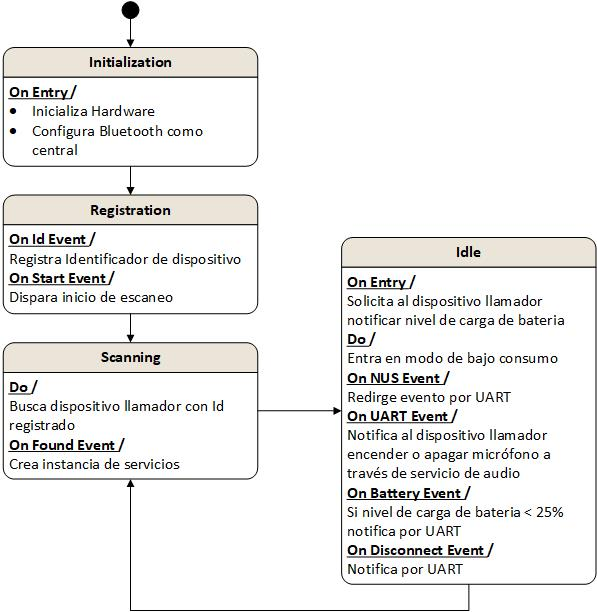
\includegraphics[scale=0.8]{./Figures/Dcentral.jpeg}
	\caption{Diagrama de bloques software central receptora}
	\label{fig:DiagramaSoftCentral}
\end{figure}

Este dispositivo es el encargado de recibir datos de todos los dispositivos llamadores, que tenga conectados. Para ello, este dispositivo se programó para que cumpla el rol de central, dentro del estándar Bluetooth BLE, de manera que este dispositivo es capaz de aceptar conexiones de hasta 7 dispositivos.

Al inicializar este dispositivo, se debe configurar el rol antes mencionado, sin embargo no empezará a escanear hasta que reciba todos los identificadores de los llamadores a los que aceptara una conexión.

Para recibir estos datos, el dispositivo iniciará la UART presente en el microcontrolador, y esperará a recibir, desde la terminal de sala, las tramas con los identificadores de todos los dispositivos llamadores que tenga asignados para cada cama, los cuales irá guardando en la RAM, en la posición que corresponda según el número de cama recibido, hasta recibir una trama final que le indica que debe empezar a buscar los dispositivos llamadores que tiene registrados. 

Este proceso de búsqueda se mantiene activo hasta que la central logra conectar a todos los dispositivos que tiene asignados. Para descartar los dispositivos no registrados, este proceso lee el identificador que le comparte el dispositivo llamador, verifica que coincida con uno de los identificadores que tiene registrados, y que esté presente el servicio de audio implementado, que también tiene un identificador único. Todo dispositivo que no cumpla con estas dos condiciones será rechazado.

Una vez que un dispositivo logra conectarse, la central receptora creará instancias de los servicios que se mencionan a continuación:

\begin{itemize}

\item Nordic Uart Service (NUS), el cual permite recibir cadenas de caracteres enviadas por los dispositivos llamadores a través de este servicio. A cada mensaje recibido, le agrega el número de cama correspondiente, según el registro de los identificadores, y lo envía al terminal de sala a través de la interfaz UART.

\item Servicio de Audio, que al igual que en el software del dispositivo llamador, se implementó uno nuevo, debido a que no existe uno disponible. Este servicio se encarga de notificar al dispositivo llamador correspondiente, cada vez que se necesita iniciar una llamada, para que este encienda su micrófono y empiece a muestrear, y le solicita notificar, cada vez que tenga una trama de audio en PCMU, la cual recibe a través este servicio. Cuando la central receptora recibe una trama, este servicio se encarga de reenviar dicha trama por la interfaz UART al terminal de sala.

\item Servicio de batería, que como se mencionó en el acápite 3.2.1 es un servicio estándar de Bluetooth LE. Cuando dicho dispositivo se conecta, este servicio le solicitará que empiece a notificar el nivel de carga de su batería. Adicionalmente, la aplicación cada vez que reciba una notificación en este servicio, verifica si está por debajo del 25\%, y de ser así, notifica este evento al terminal de sala, a través de la interfaz UART, identificando al dispositivo llamador en el que se produjo este evento

\end{itemize}

Adicionalmente a estos servicios, la central receptora verifica que todos los dispositivos que tiene conectados, permanezcan conectados. Cuando detecta que un dispositivo no está conectado, envía una notificación al terminal de sala enviando el número de cama al cual el dispositivo llamador estaba registrado.

\subsection{Software de control placa de expansión}
\label{subsec:SoftControl}

Este software es un módulo adicional al firmware que SURIX dispone para sus terminales, el mismo que no tiene una sola aplicación, por lo que dependiendo de la aplicación, este módulo se integrará o no al sistema.

El firmware del que forma parte este módulo, es un sistema implementado sobre un sistema operativo FreeRTOS, que ya tiene implementado el protocolo SIP, que permite al módulo realizar llamadas al terminal de enfermería, además de una página web de configuración del terminal.

El comportamiento general de este módulo se observa en el diagrama de flujo diseñado para su desarrollo, el mismo que se muestra en la figura \ref{fig:DiagramaSoftControl}.

\begin{figure}[htpb]
	\centering
	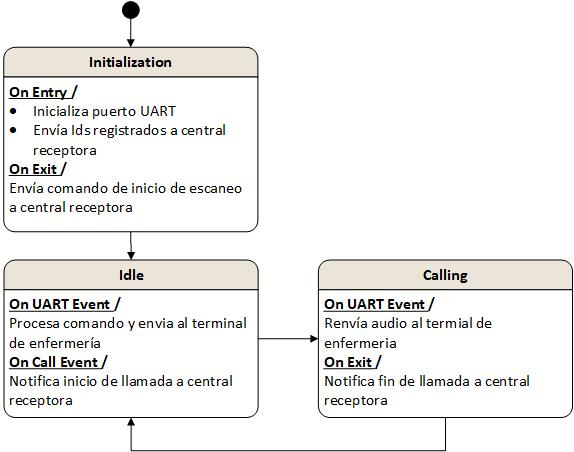
\includegraphics[scale=0.8]{./Figures/Dcontrol.jpeg}
	\caption{Diagrama de bloques software de control de la placa de expansión}
	\label{fig:DiagramaSoftControl}
\end{figure}

Cuando este módulo está presente en el sistema agrega, a la página web del sistema, un menú que le permite al usuario configurar el terminal de sala, para registrar los identificadores de los dispositivos llamadores.

Una vez que el sistema arranca, este módulo lee los identificadores de los dispositivos llamadores ingresados en la web y los envía a la central receptora, y al finalizar esta acción, envía un comando indicando a dicha central que empiece a escanear dichos dispositivos, después de lo cual, se bloquea esperando recibir novedades de esta última.

Cuando este módulo recibe una novedad, identifica el tipo de novedad y la reenvía a través de la red, ya sea local o a través de internet, al terminal de enfermería. Adicionalmente, si la novedad del paciente requiere iniciar una llamada de voz, el módulo notifica al módulo SIP que debe realizar una llamada al terminal de enfermería.

En caso de que una llamada realizada por el terminal de sala es contestada, este módulo se encarga de notificar tal evento a la central receptora para que, esta a su vez, notifique al dispositivo llamador correspondiente.

De la misma manera una vez finalizada la llamada notifica a la central receptora de tal evento para que ésta notifique al dispositivo llamador con el que se estableció la comunicación.

Durante la llamada, este módulo también se encarga de recibir los paquetes de voz de la placa receptora, y mandarlos al buffer RTP para que se transmitan en la llamada SIP.
